\section{Beyond the Standard Model: Dark matter}

\graphicspath{{1_TheoreticalBackground/Figures/DM}}

Despite its triumphs, Standard Model (SM) fails to explain many astrophysical observations~\cite{Bertone:2004pz}.
One very important question that is closely related to this thesis is the existence of dark matter (DM), which
refers to a form of matter that does not interact electromagnetically, and therefore neither emits or reflects light.
As will be explained within this section, strong evidence exists for the existence of DM, however SM
does not have any explanation about this potential form of matter.
The first subsection below aims to give a brief overview of the evidence for the existence of DM.
The following subsection covers searches of DM in particle collider experiments.

\subsection{Experimental evidence for dark matter}
\label{subsec:dm_evidence}

Evidence for the existence of DM emerged from astrophysical observations within the 20th century. In 1933,
F. Zwicky~\cite{Zwicky:1933gu} observed that galaxies in the Coma cluster are moving faster than what
is expected, requiring a larger amount of gravitational force to keep them in their orbits. Since then, the
same phenomena has been observed within individual galaxies in 1970s~\cite{Bertone:2004pz}. This can be observed
by looking at the \textit{rotation curves} of the galaxies, namely the graph of circular velocities of stars and gas
as a function of distance from the galactic center. One such rotation curve, for the NGC 6503 galaxy, is shown in
Fig.~\ref{fig:galaxy_rot_curve}.

\begin{figure}[htbp]
    \centering
    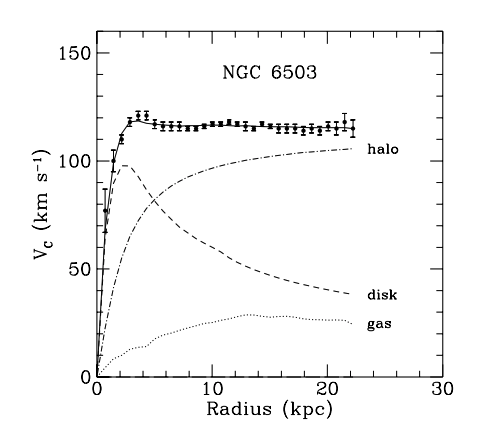
\includegraphics[width=0.7\textwidth]{galaxy_rot_curve.png}
    \caption{Rotation curve for NGC 6503 galaxy. The dashed and dotted lines represent the expected velocity profile
    from the disk (visible matter) and gas contributions, while the dash-dotted line represennts the halo (dark matter)
    contribution, required to explain the observed rotation curve. Taken from~\cite{Bertone:2004pz}.}
    \label{fig:galaxy_rot_curve}
\end{figure}

As can be observed from Fig.~\ref{fig:galaxy_rot_curve}, observed rotation curves usually exhibit a flat behavior at
large distances from the galaxy center. As shown in Fig.~\ref{fig:galaxy_rot_curve}, the contributions from the visible
disk and gas alone cannot explain the observed rotation curves. From Newtonian dynamics, the circular velocity can be
written as

\begin{equation}
    v(r) = \sqrt{\frac{G M(r)}{r}}
\end{equation}

where $M(r) = 4\pi \int \rho(r) r^{2} dr$ and $\rho(r)$ is the mass density profile. Assumming visible matter, $v(r) \propto \frac{1}{\sqrt{r}}$,
hence the fact that the rotation curves are approximately flat implies the existence of DM with $M(r) \propto r$~\cite{Bertone:2004pz}.

Another piece of evidence for the existence of DM comes from the gravitational lensing effect~\cite{Mellier:1998pk}, which refers to the
phenomena where the trajectory of light bends in the vicinity of a massive object (``deflector''), due to the curvature in 
space-time near the deflector. The dependence of this bending on the mass density of the deflector implies that gravitational
lensing can probe the mass of deflectors, making it a unique tool to probe the DM distribution in gravitational systems. In other words,
the amount of deflector mass can be measured from the amount of deflection in the trajectory of light. The amount of bending can be
deduced by measuring the angular shift of the image source $\Delta\vec{\theta}$. The amount of lensing effect can also be extracted from
the distortion of the image source. As an example, if the image source is a circular galaxy, to first approximation it can be shown that
the gravitational lensing effect transforms it into an ellipse~\cite{Mellier:1998pk}. Using the gravitational lensing technique, the
presence of large non-visible matter clusters was inferred, for example see~\cite{1988ApJ...332...75N}.

Evidence on the existence of DM is also present on the galactic scale, coming from the precise measurements of the Cosmic
Microwave Background (CMB) radiation~\cite{Hu:1995kot}. CMB is the electromagnetic radiation originating from the propagation of photons
in the early Universe, when photons decoupled from baryons. Decades of experimental effort show that the CMB follows 
the spectrum of a blackbody radiation with $T=2.726$ K, and it is nearly isotropic,
with temperature fluctuations reaching only one part in $10^{5}$ of the mean~\cite{Bertone:2004pz}.
The residual anisotropies in the CMB can be studied to extract information about the abundance of baryons and matter in the Universe. 
This is achieved by fitting
a given cosmological model with a fixed number of parameters, $N$, and finding the best-fit parameters from the peak of $N$-dimensional
likelihood. Using the data from Wilkinson Microwave Anisotropy Probe (WMAP), one can obtain the following values for the baryonic matter
density $\Omega_{b} h^{2}$ and total matter density $\Omega_{H} h^{2}$~\cite{Bertone:2004pz}:

\begin{equation}
    \Omega_{b} h^{2} = 0.024 \pm 0.01 \qquad \Omega_{M} h^{2} = 0.14 \pm 0.02
\end{equation}

where $h$ is Planck's constant. Therefore, it can be inferred that the DM relic density is $\Omega_{DM} h^2 \approx 0.12$, indicating that
predictions based on WMAP data imply that DM is more abundant compared to baryonic matter by a factor of $\approx 6$. In summary, multiple
pieces of evidence, both at galactic and cosmological scales, suggest the existence of DM. 

\subsection{Searches for dark matter}

In an effort to explain the DM observations outlined in Sec.~\ref{subsec:dm_evidence},
multiple hypotheses have been proposed, where the DM is made out of particles that are not
described by the Standard Model (very commonly called ``Beyond the Standard Model'', or ``BSM'' for short).
There are a wide range of models, where proposed types of particles include axions and weakly interacting 
massive particles (WIMPs)~\cite{Profumo:2017hqp}.

% In an effort to explain the DM observations outlined in Sec.~\ref{subsec:dm_evidence}, multiple hypotheses have been proposed. 
% Broadly speaking, one line of effort is to extend Newton's gravity and Einstein's general relativity~\cite{Famaey:2011kh}
% to try to explain discrepancies between the measured circular velocities of galactic objects and the corresponding observed mass. 

A WIMP refers to a new elementary particle which interacts via gravity\footnote{It is possible that WIMPs interact
with forces that are not described by the Standard Model, which is as weak as or weaker than the weak nuclear force.}.
Such particles are readily predicted by popular extension of the Standard Model, including 
supersymmetry~\cite{Jungman:1995df}, models with extra dimensions~\cite{Dienes:1998vh}  
and little Higgs~\cite{Arkani-Hamed:2002ikv}. In the scenario where DM is made up of WIMPs, it is possible to
detect these new particles using a number of techniques in particle detectors. 

One such technique is direct detection. The direct detection experiments look for signals from elastic scattering of DM
particles with ordinary matter. These experiments typically use detectors made out of liquid noble gases or crystals,
which are sensitive material which can generate detectable signals (such as scintillation light) in the event of a WIMP
passing through.
Such experiments include Xenon1T~\cite{XENON:2017vdw}, CRESST-II~\cite{Angloher:2011uu},
CDMSlite~\cite{SuperCDMS:2017nns}, LUX~\cite{LUX:2015abn} and PandaX-II~\cite{PandaX-II:2016vec}. At the time of writing,
no evidence has been observed of DM particles through direct detection experiments. However, very stringent constraints
on the DM-nucleuon interaction cross section have been placed as a function of hypothesized WIMP mass. XENON1T was able
to reach an upper bound of $\sigma_{DM-nucleon} < 7.7 \times 10^{47} cm^{-2}$ for a WIMP mass of $m_{DM} = 35$
GeV~\cite{XENON:2017vdw}.

Another technique for WIMP detection is the indirect detection. Indirect detection experiments look 
for evidence of WIMP self-annihilation or decay products,
such as high-energy photons or neutrinos. Hence, these experiments look for secondary products coming from the WIMP
self-interactions, as opposed to attempting to directly observe signals from a WIMP itself. One such experiment is
Fermi-LAT~\cite{Fermi-LAT:2011vow}, which is a space-based instrument that detects gamma rays. It searches for an excess
of gamma ray emission that might indicate WIMP self-annihilation or decay. Another such experiment is IceCube~\cite{Iovine:2022aiw},
which is a neutrino observatory in the South Pole. IceCube can detect high-energy neutrinos produced by cosmic-ray interactions,
and observation of an excess of neutrinos can point to WIMP self-annihilation and decay processes. Similar to direct detection results,
no evidence of WIMPs has been observed to date, but stringent limits are placed in WIMP self-annihilation cross sections. 

Finally, another technique for WIMP searches is to produce them in particle detectors, such as the Large Hadron Collider 
(LHC)\footnote{Please see Sec.~\ref{sec:large_had_collider} for the description of the LHC.}. 
With a very large proton-proton collision
center of mass energy, $\sqrt{s} = 13$ TeV\footnote{The center of mass energy for the pp collision data (2016-2018) 
used in the analysis described in this thesis is $\sqrt{s} = 13$ TeV. 
However, it should be noted that starting from 2022 data-taking, this center of mass
energy has been increased further to $\sqrt{s} = 13.6$ TeV.}, many WIMP models predict that pair production of WIMPs would be
within the kinematic reach, provided that there is some interaction between the SM sector and WIMPs. Hence, at particle colliders,
one can expect to observe the process $pp \rightarrow \chi \bar{\chi} + X$, where $\chi$ refers to the WIMP (and $\bar{\chi}$ being
it's antiparticle), and $X$ is a placeholder for other physics objects in the final state, depending on the model being considered.

One interesting class of models that is relevant to the analysis described in this thesis is the so called Higgs portal models~\cite{Argyropoulos:2021sav}.
Such models hypothesize that there are Beyond the SM interactions of the Higgs boson with the WIMPs (commonly also called ``dark sector''),
and proton-proton colliders are excellent machines to probe such interactions of the Higgs boson through its decay products, i.e. 
$H \rightarrow \chi \bar{\chi}$, because of the large rates of Higgs bosons being produced. These models are discussed in more detail in the
following section, where Sec.~\ref{subsec:higgs_portal_theory} gives an overview of the theory, and Sec.~\ref{subsec:exp_signatures} gives an overview
of the experimental signatures expected in proton-proton collisions.  




